%%%%%%%%%%%%%%%%%%%%%%%%%%%%%%%%%%%%%%%%%%%%%%
% An example of a lab report write-up.
%%%%%%%%%%%%%%%%%%%%%%%%%%%%%%%%%%%%%%%%%%%%%% 
% This is a combination of several labs that I have done in the past for 
% Computer Engineering, so it is not to be taken literally, but instead used as 
% a great starting template for your own lab write up.  When creating this 
% template, I tried to keep in mind all of the functions and functionality of 
% LaTeX that I spent a lot of time researching and using in my lab reports and 
% include them here so that it is fairly easy for students first learning LaTeX
% to jump on in and get immediate results.  However, I do assume that the 
% person using this guide has already created at least a "Hello World" PDF 
% document using LaTeX (which means it's installed and ready to go). 
%
% My preference for developing in LaTeX is to use the LaTeX Plugin for gedit in 
% Linux.  There are others for Mac and Windows as well (particularly MikTeX).  
% Another excellent plugin is the Calc2LaTeX plugin for the OpenOffice suite.  
% It makes it very easy to create a large table very quickly.  
%
% Professors have different tastes for how they want the lab write-ups done, so 
% check with the section layout for your class and create a template file for 
% each class (my recommendation).
%
% Also, there is a list of common commands at the bottom of this document.  Use
% these as a quick reference.  If you'd like more, you can view the "LaTeX Cheat
% Sheet.pdf" included with this template material. 
%
% (c) 2009 Derek R. Hildreth <derek@derekhildreth.com> http://www.derekhildreth.com 
% This work is licensed under the Creative Commons Attribution-NonCommercial-ShareAlike License. To view a copy of this license, visit http://creativecommons.org/licenses/by-nc-sa/1.0/ or send a letter to Creative Commons, 559 Nathan Abbott Way, Stanford, California 94305, USA.
%%%%%%%%%%%%%%%%%%%%%%%%%%%%%%%%%%%%%%%%%%%%%%
\documentclass[aps,letterpaper,10pt]{revtex4}
\input kvmacros % For Karnaugh Maps (K-Maps)

\usepackage{endnotes}
\usepackage{graphicx} % For images
\usepackage{float}    % For tables and other floats
\usepackage{verbatim} % For comments and other
\usepackage{amsmath}  % For math
\usepackage{amssymb}  % For more math
\usepackage{fullpage} % Set margins and place page numbers at bottom center
\usepackage{listings} % For source code
\usepackage{gensymb} %ohms and shit
\usepackage{subfig}   % For subfigures
\usepackage[usenames,dvipsnames]{color} % For colors and names
\usepackage[pdftex]{hyperref}           % For hyperlinks and indexing the PDF
\hypersetup{ % play with the different link colors here
    colorlinks,
    citecolor=blue,
    filecolor=blue,
    linkcolor=blue,
    urlcolor=blue % set to black to prevent printing blue links
}
\usepackage{tikz} \usepackage{circuitikz} \usepackage{siunitx}

\definecolor{mygrey}{gray}{.96} % Light Grey
\lstset{ 
	language=[ISO]C++,              % choose the language of the code ("language=Verilog" is popular as well)
   tabsize=3,							  % sets the size of the tabs in spaces (1 Tab is replaced with 3 spaces)
	basicstyle=\tiny,               % the size of the fonts that are used for the code
	numbers=left,                   % where to put the line-numbers
	numberstyle=\tiny,              % the size of the fonts that are used for the line-numbers
	stepnumber=2,                   % the step between two line-numbers. If it's 1 each line will be numbered
	numbersep=5pt,                  % how far the line-numbers are from the code
	backgroundcolor=\color{mygrey}, % choose the background color. You must add \usepackage{color}
	%showspaces=false,              % show spaces adding particular underscores
	%showstringspaces=false,        % underline spaces within strings
	%showtabs=false,                % show tabs within strings adding particular underscores
	frame=single,	                 % adds a frame around the code
	tabsize=3,	                    % sets default tabsize to 2 spaces
	captionpos=b,                   % sets the caption-position to bottom
	breaklines=true,                % sets automatic line breaking
	breakatwhitespace=false,        % sets if automatic breaks should only happen at whitespace
	%escapeinside={\%*}{*)},        % if you want to add a comment within your code
	commentstyle=\color{BrickRed}   % sets the comment style
}

% Make units a little nicer looking and faster to type
\newcommand{\Hz}{\textsl{Hz}}
\newcommand{\KHz}{\textsl{KHz}}
\newcommand{\MHz}{\textsl{MHz}}
\newcommand{\GHz}{\textsl{GHz}}
\newcommand{\ns}{\textsl{ns}}
\newcommand{\ms}{\textsl{ms}}
\newcommand{\s}{\textsl{s}}

%for ease of entry
\newcommand{\voltage}[1]{$V_{#1}$}
\newcommand{\current}[1]{$I_{#1}$}
\newcommand{\resistance}[1]{$R_{#1}$}
\newcommand{\kiloohm}[1]{\SI{#1}{\kilo\ohm}}
\newcommand{\ohms}[1]{\SI{#1}{\ohm}}

%spacing
%Custom indenting
\newcommand{\single}{\hspace*{0.5cm}}
\newcommand{\double}{\hspace*{1cm}}


% TITLE PAGE CONTENT %%%%%%%%%%%%%%%%%%%%%%%%
% Remember to fill this section out for each
% lab write-up.
%%%%%%%%%%%%%%%%%%%%%%%%%%%%%%%%%%%%%%%%%%%%%
\newcommand{\labname}{EE 119c Project Proposal}
\newcommand{\descript}{FPGA-Based Pitch Detector and Tuner}
\newcommand{\authorname}{Dan Pipe-Mazo}
\newcommand{\professor}{Glen George}
\newcommand{\classno}{Spring 2013}
% END TITLE PAGE CONTENT %%%%%%%%%%%%%%%%%%%%


\begin{document}  % START THE DOCUMENT!


% TITLE PAGE %%%%%%%%%%%%%%%%%%%%%%%%%%%%%%%%%%%%%%
% If you'd like to change the content of this,
% do it in the "TITLE PAGE CONTENT" directly above
% this message
%%%%%%%%%%%%%%%%%%%%%%%%%%%%%%%%%%%%%%%%%%%%%%%%%%%
\begin{titlepage}
\begin{center}
{\LARGE \textsc{\labname:} \\ \vspace{4pt}}
{\Large \textsc{\descript} \\ \vspace{4pt}} 
\rule[13pt]{\textwidth}{1pt} \\ \vspace{150pt}
{\large By: \authorname \\ \vspace{10pt}
Instructor: \professor \\ \vspace{10pt}
California Institute of Technology \\ \vspace{10pt}
\classno \\ \vspace{10pt}}
\end{center}
\end{titlepage}
% END TITLE PAGE %%%%%%%%%%%%%%%%%%%%%%%%%%%%%%%%%%

%%%%%%%%%%%%%%%%%%%%%%%%%%%%%%
%%%%%%%%%%%%%%%%%%%%%%%%%%%%%%
\section{Overview}

This project will be a digital, real-time pitch detection and tuning system. The system will be able to determine the dominant frequency of any audio signal between 15 and 5,000Hz (between musical notes $C_0$ and $D^\#_8$) played to within 1Hz and 0.1\% accuracy on all notes in the range. The detected frequency will be displayed in floating-point form on a display to the user, as well as the closest musical note and an indication of how far the detected frequency differs from the closest note. This allows the user to manually tune an instrument, using the display of the system to identify when the frequency of the note played matches the desired note. \\ 

The system will employ several techniques to maximize the accuracy of its readings. The first technique is sampling frequency variation. In order to maintain a small sample size and minimize logic, 5 different sampling frequencies are employed to cover all notes in the 15 to 5,000 Hz range. These frequencies were chosen to minimize logic and also maintain 1Hz and 0.1\% error thresholds for all pitches in the range. The system also employs background noise-canceling techniques and a variable gain audio amplifier to ensure that the measurements which the sigma-delta converter makes are able to use the op-amps' full dynamic range and thereby increase accuracy. \\

In order to detect pitch, the system loosely employs the method developed by Dubnowski, Schafer and Rabiner\endnote{\textbf{Real-Time Digital Hardware Pitch Detector}, Dubnowski,  Shafer and Rabiner. Published February 1976 in Volume ASSP-24, No. 1 of \textit{IEEE Transactions on Acoustics, Speech and Signal Processing}. Currently available at \url{http://cronos.rutgers.edu/~lrr/Reprints/095_hardware\%20pitch\%20detector.pdf}}. First employs center and infinite peak clipping to transform the incoming audio signal into either a 1, -1 or 0. This is performed by determining a clipping threshold such that approximately 20\% of the positive data in a given sample is above the upper threshold, and 20\% of the negative data is below the lower threshold. If the data lies above the upper threshold, it is stored as a 1. If the data lies below the lower threshold, it is stored as a 0, and if the data is between the two thresholds, it is stored as a 0. After clipping the data, autocorrelation is applied to the stored audio samples to look for a peak. When the peak is found at a particular sample, j, in the sampled audio, the corresponding frequency is equal to the sampling frequency divided by j.\\

The system will also have automatic tuning capability--initially for guitars but expandable to any instrument--through the use of a stepper motor and specialized instrument attachment. For a guitar, the driveshaft of the stepper motor will be directly attached to a socket which fits on a standard acoustic guitar tuning knob. When the user selects for the unit to automatically tune a string of a guitar, the user will input the desired frequency or note for the string to the system, and will only need to pluck the string once. The system, with its fast pitch-detection will continuously loop detecting the frequency of the string and turning the stepper motor until the frequency of the string matches the desired frequency.\\ 

The above functionality can be expanded through the use of different stepper motor attachments to tune a wide variety of instruments. The high torque and precision of the stepper motor will allow for accurate and precise tuning.

%%%%%%%%%%%%%%%%%%%%%%%%%%%%%
%%%%%%%%%%%%%%%%%%%%%%%%%%%%%%
\section{Operational Description}
Audio signal is delivered to the FPGA after a series of mainly digitally-controlled analog operations. Audio comes in through the microphone and is then through a digitally controlled subtractor. This subtractor is used to subtract background noise. When the system prepares to detect pitch, it adjusts this subtractor so that the incoming audio signal does not have significant noise on it. The system adjusts this subtracter by changing the value of a resistor in the subtractor circuit with a digitally controlled potentiometer.\\

Once the audio has passed through the subtractor, it is fed into a digitally controlled, variable gain amplifier. This amplifier serves two purposes: ensure that the full dynamic range of the op-amps is utilized while also performing the center clipping. The system will adjust the gain on the amplifier until approximately 10\%of all samples are at the maximum output of the sigma-delta converter and 10\% of all samples are at the minimum output of the sigma-delta converter. By being able to digitally control this amplifier to perform the clipping, it is not necessary to store full converted samples to perform clipping level calculations, thereby saving a massive amount of space. \\

After being clipped, the audio is sent through a low-pass filter with a corner frequency at 20KHz. This allows for all audible signals to pass through, though some are outside of the specified range of operation for the unit. Even though outside of the range of operation, these signals will still be calculated with less than 1\% error, though 1Hz accuracy cannot be guaranteed. \\

After being filtered, the audio is sent through an analog to digital converter. As mentioned in the overview, the analog to digital converter will run at five different sampling frequencies in order to ensure 0.1\% and 1Hz accuracy within the range of 50 to 5000Hz. The sampling rates at which the sigma-delta converter will run are 50Msps, 25Msps, 6.25Msps, 1.5625Msps and 195.3125Ksps. At each sampling frequency, a total of 15000 samples will be taken. The sampling frequencies were chosen to meet the following criteria:
\begin{enumerate}
\item Minimize 1-bin error. For an audio sample of a given frequency, it will most likely not be on the exact boundary of an autocorrelation bin, and thus some error will be introduced when the autocorrelation peak is detected at one of the binned frequencies. In order to calculate maximum error, the case where a signal was placed into one bin too high or too low for its frequency. 1-bin error is also analogous to the frequency space between bins. The 1-bin error was computed for all frequencies in the 50 to 5000Hz range, and is displayed in Figure \ref{fig:error} below in two ways: in absolute frequency (Hz) and as a percentage error. 1-Bin error was kept to under 0.5Hz, allowing for 2 bins of error to add to less than 1Hz. Error is computed using the following formulas:
$$ 1-bin~error(in~Hz) = (\frac{1}{m - 1} - \frac{1}{m})\times sampling~frequency$$
$$ m = \frac{sampling~frequency}{audio~frequency}$$
where m is the discretized bin number of the primary frequency for any audio sampled at a given sampling frequency. When looking at the plots in Figure \ref{fig:error}, the discontinuities are due to changing of the sigma-delta converter sampling frequency. For correlations between audio frequency to detect and sigma-delta sampling frequency, please see Section IV, Algorithm Runtime. 
\item Minimize FPGA space required. For each sample, two bits of storage and a 12-bit up/down counter are necessary (implemented using 4-gate J-K FFs and 3 additional logic gates for up/down functionality per bit). Thus, minimizing sample size is crucial. Also, the runtime of the algorithm within the FPGA once samples are collected is dependent on the sample size, since autocorrelation requires a sample size length addition cycle. 
\item Minimize total measurement time. The sampling frequencies are scanned through from highest to lowest. This means that for a low-frequency signal, all higher frequencies must be scanned through before getting to the lowest sampling frequency and being able to identify the signal. The less sampling frequencies which are employed, the less total time is wasted before identifying low-frequency signals. 
\item Evenly distribute sampling error. The sampling frequencies were chosen to provide the best spectrum coverage while ensuring that error, while minimized throughout the system, was as consistent as possible. 
\end{enumerate}

\begin{figure}[H]
  \centering
  \subfloat[1-Bin error in Hz]{\label{fig:Per4}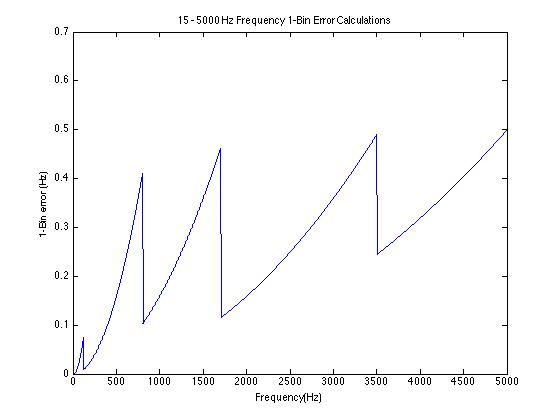
\includegraphics[width=0.8\textwidth]{error_in_hz.jpg}} \\                
  \subfloat[1-Bin error in percent]{\label{fig:Per5}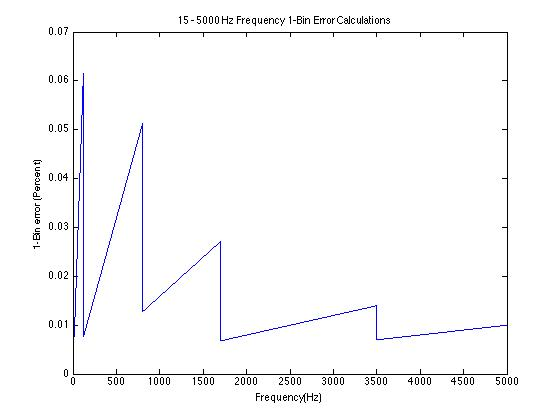
\includegraphics[width=0.8\textwidth]{error_in_percent.jpg}}
  \caption{1-Bin error calculations.}
  \label{fig:error}
\end{figure}
After passing through the sigma-delta converter, the data is passed into the FPGA where it is first assigned a 1, 0 or -1 value and stored. After all samples are stored, autocorrelation is run. The autocorrelation algorithm employed is:
$$R_x(m) \sum_{n = 0}^{14999 - m}{x(n)\times x(n + m)~~~~~~~~~~~~~~~~~~~m = 0, 1, 2, 3, ... 14999}$$
Where $R_x(m)$ is the autocorrelation value for the $m^{th}$ bin of frequencies, and $x(k)$ is the $k^{th}$ sample collected in an input. Since all  $x(k)$ values are 2-bit signed values,  $$x(n)\times x(m) = (x(n)_1~xor~x(m)_1 )~\&~( x(n)_0~and~x(m)_0 )$$
The multiplication can be performed in two gates per value. Once the multiplication is performed, a 12-bit incrementer-decrementer is either incremented, decremented or kept the same based on the result of the multiplication. 12 bits are necessary since a perfect autocorrelation score can be obtained when all nonzero elements of the signal add to the autocorrelation value and only 20\% of the data is clipped to be nonzero, thus leaving $0.2*15000 = 3000$ as the perfect autocorrelation score with properly executed clipping. The incrementer-decrementer is implemented using one 4-gate J-K flip-flop and 3 additional up/down logic gates per bit, meaning each incrementer-decrementer adds 84 gates to the design. The autocorrelation algorithm will be executed in 15000 clocks, shifting around values as necessary. An additional 2 bits of DFF storage (6 gates each) will be needed as well to aid in the shifting and multiplication. All in all, then, the autocorrelation algorithm adds 96 gates per sample to the FPGA. \\

Once the autocorrelation is completed, the FPGA will run a peak detection algorithm on the autocorrelation values to see if a peak is exhibited. If no peak is exhibited, the sampling frequency was too high to fit the entire period of the input audio signal. The next lower sampling frequency will then be used to collect more data and the process will be repeated. If a peak is detected, its frequency is calculated using the formula:
$$audio~frequency = \frac{sampling~frequency}{m}$$ where m is the same as from $R_x(m)$ i.e. the sample number at which the peak is detected. \\

The frequency detected will then be sent to the control unit of the FPGA to be output on the display. If the user selected a tuning mode, the display will also show the closest musical note to the detected frequency, as well as a measure of how far from the desired note the detected frequency is. \\

If the user selected automatic tuning, the frequency detected will be subtracted from the desired frequency, and the difference will be sent to the motor control unit within the FPGA. The motor control unit will then calculate the number of steps by which to rotate the stepper motor based on the frequency difference. The motor unit will then rotate the stepper motor, and pitch detection will be re-performed. This process will be continued until the string is tuned (to a margin of error determined by the experimentally determined accuracy of the auto-tuning system).\\

The FPGA has a control unit which handles monitoring user input, dealing with the display, implanting control logic to interface between the various aspects of the sampling and autocorrelation algorithms, controlling the digital potentiometers in the analog circuitry and supplying the sample clock to the sigma-delta converter. Since the converter will be running at a maximum of 50MHz, the FPGA must run at 50MHz or higher. All other sample clocks are simple power of 2 divisions of a 50MHz clock.\\

%%%%%%%%%%%%%%%%%%%%%%%%%%%%%
%%%%%%%%%%%%%%%%%%%%%%%%%%%%%%
\section{FPGA Size Estimate}
Some numbers relating to FPGA size were stated in the Operational Description section. Essentially, the size of the FPGA is dictated by the size of the initial clipped sample storage and the size of the autocorrelation circuitry. Each clipped sample needs to be stored in 2 bits of RAM. Assuming that the RAM is implemented as DFFs (6 gates each), then initial sample storage will consume $15,000\times(6 \times 2) = 180,000$ gates.\\

Autocorrelation will take another 2 bits of storage, as well as 12 bits of incrementer-decrementer per sample. The incrementer-decrementer will be implemented using a J-K flip-flop (4 gates) and increment/decrement control logic (3 gates) per bit. This sums to 96 gates per sample, which totals to $15,000\times96 = 1,440,000$ gates.\\

Summing these two numbers yields 1.62 million gates from storage and autocorrelation alone. The sigma-delta converter, control unit and remaining logic will bring the total gate count to approximately \textbf{2 million gates}. If space winds up being an issue, more sampling frequencies can be introduced and the sample size can be decreased at the cost of total overall runtime, since it will take longer time to detect lower frequencies. 

%%%%%%%%%%%%%%%%%%%%%%%%%%%%%
%%%%%%%%%%%%%%%%%%%%%%%%%%%%%%
\section{Algorithm Runtime}
The unit takes 15,000 sample points at the sampling frequency. This is:
\begin{itemize}
\item 0.3ms at 50Msps (5KHz to 3.5KHz signals)
\item 0.6ms at 25Msps (3.5KHz to 1.7KHz signals)
\item 2.4ms at 6.25Msps (1.7KHz to 800Hz signals)
\item 9.6ms at 1.5625Msps (800Hz to 120Hz signals)
\item 76.8ms at 195.3125 Ksps (120Hz to 15Hz signals)
\end{itemize}

After sampling, the unit first performs clipping level adjustments, if necessary. If a clipping level adjustment is necessary, the data must be re-sampled. The ideal approximations below assume that an appropriate clipping level has already been set. Once the samples have been collected, the system performs autocorrelation in 15,000 system clocks. Assuming a system clock of 50MHz, this is 0.3ms. The system then performs peak detection in another 15,000 system clocks, taking another 0.3 ms If a peak is detected, then the algorithm is done. If not, the system samples at the next lowest frequency and repeats this process until it finds a peak. The autocorrelation and peak detection process is then a constant 0.6ms regardless of frequency. Thus, the algorithm runtime, based on input frequency, are as follows: \\

\noindent \textbf{5KHz to 3.5KHz signals}: \\
0.3ms sampling + 0.6ms detection = \textbf{0.9ms}\\

\noindent \textbf{3.5KHz to 1.7KHz signals}: \\
0.3ms sampling + 0.6ms detection + 0.6ms sampling + 0.6ms detection = \textbf{2.1ms}\\

\noindent \textbf{1.7KHz to 800Hz signals}: \\
0.3ms sampling + 0.6ms detection + 0.6ms sampling + 0.6ms detection + 2.4ms sampling + 0.6ms detection = \textbf{5.1 ms}\\

\noindent \textbf{800Hz to 120Hz signals}: \\
0.3ms sampling + 0.6ms detection + 0.6ms sampling + 0.6ms detection + 2.4ms sampling + 0.6ms detection + 9.6ms sampling + 0.6ms detection = \textbf{15.3 ms}\\

\noindent \textbf{120Hz to 15Hz signals}: \\
0.3ms sampling + 0.6ms detection + 0.6ms sampling + 0.6ms detection + 2.4ms sampling + 0.6ms detection + 9.6ms sampling + 0.6ms detection + 76.8ms sampling + 0.6ms detection = \textbf{92.7 ms}\\


%%%%%%%%%%%%%%%%%%%%%%%%%%%%%
%%%%%%%%%%%%%%%%%%%%%%%%%%%%%%
\section{Functional Specification}
The FPGA-Based Pitch Detector and Tuner will display the frequency of any audible tone. It will display the closest musical note (if appropriate) to the audible tone detected, and will display an indication of how far away from the perfect frequency for the closest note the audible tone is. It also has the capability to automatically tune an instrument using a stepper motor to turn a tuning knob. The user can tell the system exactly which note or frequency to tune to, play the string to be tuned once, and by the time that the string has stopped vibrating it will be perfectly in tune. \\

\noindent \textsc{\large Features}\\

\begin{itemize}
\item LCD Display shows detected frequency, closest musical note and margin of error from closest musical note. 
\item FPGA-based sigma-delta converter sampling at speeds up to 50Msps.
\item Frequency identification accuracy within 1Hz and 0.1\% for all values between 15Hz and 5000Hz ( $C_0$ to $D^\#_8$).
\item Stepper motor with 200 steps per revolution and micro stepping capability allows for precision tuning while also having enough torque to crank stiff tuning knobs. 
\item Precise, digitally-controlled amplification and background-noise cancellation prevents erroneous output from displaying on the screen and increases the accuracy of the system.
\end{itemize}

\noindent \textsc{\large Inputs}\\

\begin{itemize}
\item Pushbutton rotary encoder and four input keys (up, down, left, right) for navigating through the menus and features of the user interface
\item Microphone to capture audio
\end{itemize}

\noindent \textsc{\large Outputs}\\

\begin{itemize}
\item LCD screen displays exact frequency of tone played, closest note, and margin of error from closest note
\item If automatic tuning is activated, stepper motor will rotate to tune instrument
\end{itemize}

\noindent \textsc{\large Major Hardware}\\

The FPGA-Based pitch detector and Tuner will run on a Xilinx FPGA. The FPGA will need to be between 2 million and 4 million gates, as discussed in the FPGA Size Estimate section above. \\

In addition to the FPGA, the pitch detector will utilize:
\begin{itemize}
\item A sigma-delta converter with $\geq 20$ bits of resolution capable of sampling at speeds greater than 50Msps. 
\item An analog low-pass filter (10KHz corner frequency), in order to allow for faster pitch calculation times. 
\item Analog voltage subtractor and amplifying circuitry controlled by digital potentiometers in order to subtract out background noise and perform clipping. 
\item A LCD or similar display.
\item A stepper motor with $\geq 200$ steps per revolution, accompanied by stepper motor driver chips. 
\end{itemize}

\noindent \textsc{\large User Interface}\\

The FPGA-Based Pitch Detector and tuner will feature a LCD which the act to both display information to the user and take input from the user. The LCD and accompanying switches and rotary encoder will allow the user to select a mode to operate the device in from one of the following modes:
\begin{enumerate}
\item \textbf{General Pitch Detection}: Have the pitch detector continuously run and display the current pitch of audio input. Pitch shown in to an appropriate number of decimal places. 
\item \textbf{Tuning}: Choose a note in the range of  $C_0$ to $D^\#_8$ and view how close to in tune the audio input is to the desired note. Real-time feedback allows for easy and quick manual tuning. Pitch shown in Hz to an appropriate number of decimal places. Visual feedback as to how far out of tune from the desired note is provided on-screen.
\item \textbf{Automatic Tuning}: For any open-string guitar tuning, choose a note, attach the stepper motor unit to the tuning knob, pluck the note once, and by the time time note finishes playing, it will be perfectly in tune. 
\end{enumerate}

\noindent \textsc{\large Limitations}\\

Current limitations for the device are:
\begin{itemize}
\item Can only detect frequencies from 15Hz to 5KHz within 0.1\% and 1Hz error margins
\item Automatic tuning only works for guitars
\item Not able to detect multiple notes being played at the same time
\end{itemize}
All of the above limitations can potentially be solved through further development, but are not included in the base design of the project. 

\newpage
\section{Block Diagram}
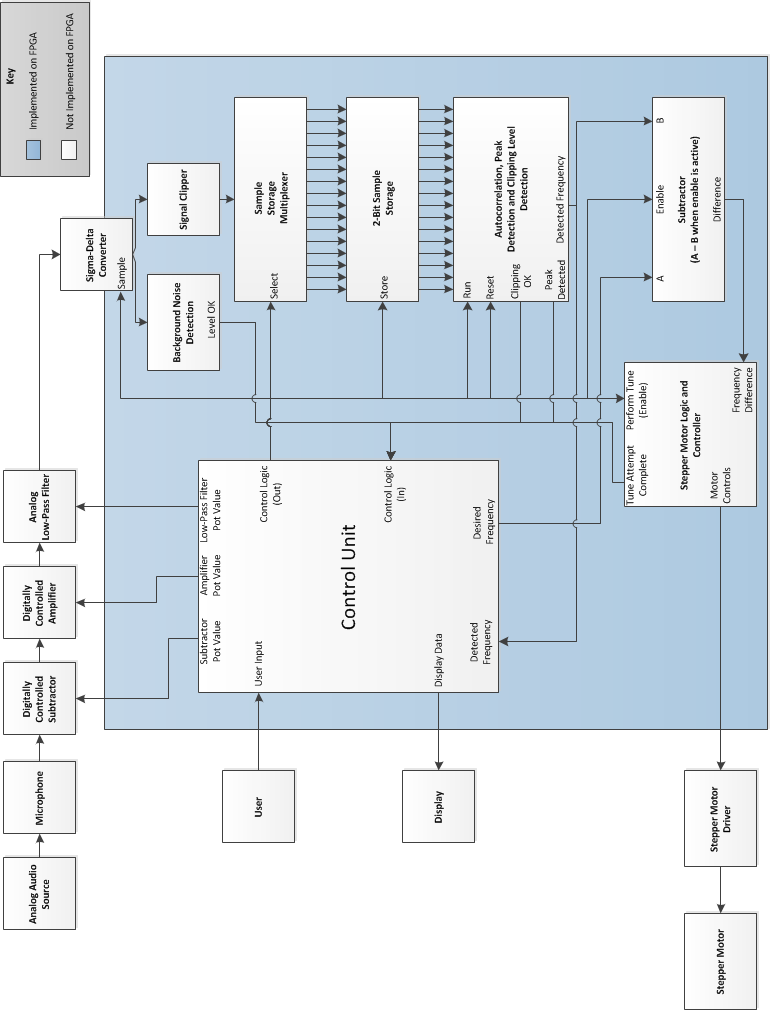
\includegraphics[width=\textwidth]{EE119c_block_diagram.png}


\section{Demonstration}
The project will be demonstrated with the following tests:
\begin{enumerate}
\item Use a function generator to generate tones in the range of 15 to 5000 Hz, and view the display of the pitch detector to verify functionality. Ensure that 1Hz or 0.1\% error margins are obeyed, whichever margin is tighter. 
\item Use a function generator to generate tones close to but not exactly that of E2, A2, D3, G3, B3 and E4, the 6 open strings of the guitar, and use the information on the LCD of the pitch detector to manually tune the function generator to precise frequencies. 
\item Untune a guitar string and use the pitch detector's automatic tuning motor to automatically tune the string in a single pluck.
\end{enumerate}

\section{Schedule}
Weekly milestones are proposed as follows:
\begin{enumerate}
\item Choose all hardware and order/sample parts. Completely flesh out block diagrams, detailing all signals and control logic.
\item Write control unit VHDL code
\item Write sampling and sigma-delta code, breadboard analog circuitry
\item Write autocorrelation and peak detection code
\item Write motor control code, breadboard entire design
\item Integrate all code together, design any PCBs needed
\item Write VHDL test bench
\item Test using test bench and fix bugs
\item Assemble PCBs and final hardware design, more testing and debugging
\item Final testing, presentation and documentation
\end{enumerate}
%%%%%%%%%%%%%%%%%%%%%%%%%%%%%%
%%%%%%%%%%%%%%%%%%%%%%%%%%%%%%
	


%%%%%%%%%%%%%%%%%%%%%%%%%%%%%%
%%%%%%%%%%%%%%%%%%%%%%%%%%%%%


%%%%%%%%%%%%%%%%%%%%%%%%%%%%%%
%%%%%%%%%%%%%%%%%%%%%%%%%%%%%%

\theendnotes
\end{document} % DONE WITH DOCUMENT!


%%%%%%%%%%
PERSONAL FAVORITE LAB WRITE-UP STRUCTURE
%%%%%%%%%%
\section{Introduction}
	% No Text Here
	\subsection{Purpose}
		% Lab objective
	\subsection{Equipment}
		% Any and all equipment used (specific!)
	\subsection{Procedure}
		% Overview of the procedure taken (not-so-specific!)
\newpage
\section{Schematic Diagrams}
	% Any schematics, screenshots, block
   % diagrams used.  Possibly photos or
	% images could go here as well.
\newpage
\section{Experiment Data}
	% Depending on lab, program code would be 
	% included here without the Estimated and 
	% Actual Results.
	\subsection{Estimated Results}
		% Calculated. What it should be.
	\subsection{Actual Results}
		% Measured.  What it actually was.
\newpage
\section{Discussion \& Conclusion}
	% 3 Paragraphs:
		% Restate the objective of the lab
		% Discuss personal trials, errors, and difficulties
		% Conclude the lab


%%%%%%%%%%%%%%%%
COMMON COMMANDS:
%%%%%%%%%%%%%%%%
% IMAGES
begin{figure}[H]
   \begin{center}
      \includegraphics[width=0.6\textwidth]{RTL_SCHEM.png}
   \end{center}
\caption{A screenshot of the RTL Schematics produced from the Verilog code.}
\label{RTL}
\end{figure}

% SUBFIGURES IMAGES
\begin{figure}[H]
  \centering
  \subfloat[LED4 Period]{\label{fig:Per4}\includegraphics[width=0.4\textwidth]{period_led4.png}} \\                
  \subfloat[LED5 Period]{\label{fig:Per5}\includegraphics[width=0.4\textwidth]{period_led5.png}}
  \subfloat[LED6 Period]{\label{fig:Per6}\includegraphics[width=0.4\textwidth]{period_led6.png}}
  \caption{Period of LED blink rate captured by osciliscope.}
  \label{fig:oscil}
\end{figure}

% INSERT SOURCE CODE
\lstset{language=Verilog, tabsize=3, backgroundcolor=\color{mygrey}, basicstyle=\small, commentstyle=\color{BrickRed}}
\lstinputlisting{MODULE.v}

% TEXT TABLE
\begin{table}
\begin{center}
\begin{tabular}{|l|c|c|l|}
	x & x & x & x \\ \hline
	x & x & x & x \\
	x & x & x & x \\ \hline
\end{tabular}
\caption{Caption}
\label{label}
\end{center}
\end{table}

% MATHMATICAL ENVIRONMENT
$ 8 = 2 \times 4 $

% CENTERED FORMULA
\[  \]

% NUMBERED EQUATION
\begin{equation}
	
\end{equation}

% ARRAY OF EQUATIONS (The splat supresses the numbering)
\begin{align*}
	
\end{align*}

% NUMBERED ARRAY OF EQUATIONS
\begin{align}
	
\end{align}

% ACCENTS
\dot{x} % dot
\ddot{x} % double dot
\bar{x} % bar
\tilde{x} % tilde
\vec{x} % vector
\hat{x} % hat
\acute{x} % acute
\grave{x} % grave
\breve{x} % breve
\check{x} % dot (cowboy hat)

% FONTS
\mathrm{text} % roman
\mathsf{text} % sans serif
\mathtt{text} % Typewriter
\mathbb{text} % Blackboard bold
\mathcal{text} % Caligraphy
\mathfrak{text} % Fraktur

\textbf{text} % bold
\textit{text} % italic
\textsl{text} % slanted
\textsc{text} % small caps
\texttt{text} % typewriter
\underline{text} % underline
\emph{text} % emphasized

\begin{tiny}text\end{tiny} % Tiny
\begin{scriptsize}text\end{scriptsize} % Script Size
\begin{footnotesize}text\end{footnotesize} % Footnote Size
\begin{small}text\end{small} % Small
\begin{normalsize}text\end{normalsize} % Normal Size
\begin{large}text\end{large} % Large
\begin{Large}text\end{Large} % Larger
\begin{LARGE}text\end{LARGE} % Very Large
\begin{huge}text\end{huge}   % Huge
\begin{Huge}text\end{Huge}   % Very Huge


% GENERATE TABLE OF CONTENTS AND/OR TABLE OF FIGURES
% These seem to have some issues with the "revtex4" document class.  To use, change
% the very first line of this document to "article" like this:
% \documentclass[aps,letterpaper,10pt]{article}
\tableofcontents
\listoffigures
\listoftables

% INCLUDE A HYPERLINK OR URL
\url{http://www.derekhildreth.com}
\href{http://www.derekhildreth.com}{Derek Hildreth's Website}

% FOR MORE, REFER TO THE "LINUX CHEAT SHEET.PDF" FILE INCLUDED!
